\chapter[Integração dos Projetos]{Integração dos Projetos}
\label{chap:inte}
	
	Neste capítulo são apresentados os principais testes de integração necessários para construção final da bancada. Para a integração de todos os produtos, algumas áreas foram designadas para fazer sua integração de forma conjunta, a Figura \ref{inte00} apresenta a execução dos testes de forma cronológica.

	\begin{figure}[htpb]
		\centering
		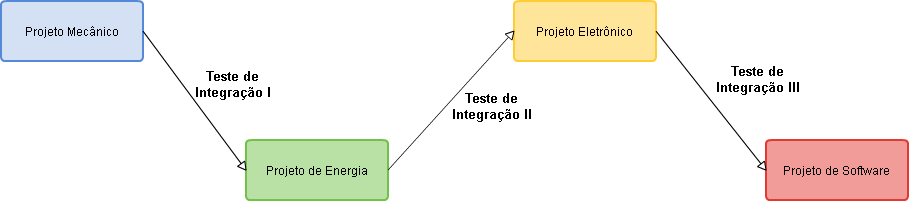
\includegraphics[width=1\textwidth]{inte00}
		\caption{Integrações dos Projetos Mecânico-Energia-Eletrônico-Software}
		\label{inte00}
	\end{figure}

	Na seção \ref{sec:inte11} é apresentada a integração entre os produtos das Equipe de Mecânica e Energia. Já na seção \ref{sec:inte22} é apresentada a integração entre os produtos das Equipes de Energia e Eletrônica. Na seção \ref{sec:inte33} é apresentada a integração entre os produtos das Equipes de Eletrônica e de Software. Por fim, na seção \ref{sec:inte44} é apresentado o custo total do projeto.

	\section{Teste de Integração I - Equipes de Mecânica e Energia}
	\label{sec:inte11}

		Como se trata de uma equipe composta por cinco engenharias, a integração é fundamental, e nessa fase do projeto, foi importantíssima. 
		
		Foi necessária nessa fase a integração dos produtos gerados pelo projeto de Energia com os do projeto Mecânico. Definiu-se então que seria realizado um teste de integração, com amortecedor e caixa de redução acoplados ao motor elétrico. O objetivo desta integração foi de garantir que o motor elétrico seria capaz de movimentar o aparato mecânico da bancada.
		
		Para realizar o teste de integração entre Mecânica e Energia, foram necessários os seguintes requisitos:

		\begin{itemize}
			\item Detalhamento da planta de fixação do motor disponibilizado pela Equipe de Energia;
			\item Detalhamento da disposição do amortecedor disponibilizado pela Equipe Mecânica;
			\item Base de acoplamento do motor na bancada definido e desenhado no CATIA; 
			\item Disponibilização de amortecedores a serem usados para o teste;
			\item Esquema mecânico de ligação entre motor e caixa de redução já definidos(polias e correias).
		\end{itemize}

		A Figura a seguir apresenta o procedimento necessário para execução do teste.

		\begin{figure}[htpb]
			\centering
			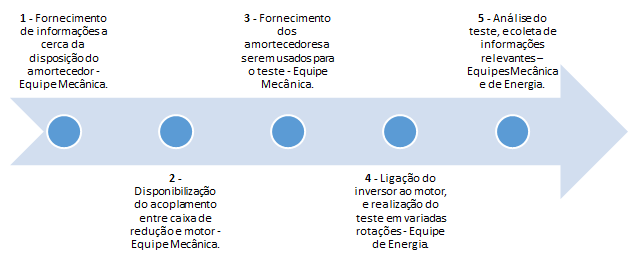
\includegraphics[width=1\textwidth]{inte01}
			\caption{Procedimento para realização do Teste de Integração Mecanica-Energia}
			\label{inte01}
		\end{figure}


	\section{Teste de Integração II - Equipes de Energia e Eletrônica}
	\label{sec:inte22}

		Os projetos das Equipes de Energia e Eletrônica foram integralizados de forma a estabelecer a comunicação entre os respectivos módulos operacionais propostos por tais áreas, a partir da integração entre o controle de velocidades do motor com o controle da entrada e saída de dados.
		
		A integração feita entre os dois projetos foi projetada de modo a permitir a comunicação entre o sistema eletrônico e o inversor de frequência dimensionado, com o objetivo de permitir o controle de velocidades do motor de indução e, consequentemente, as velocidades do amortecedor durante o teste.

		
		Para a realização do teste, foram considerados os seguintes passos:

		\begin{itemize}
			\item Conhecer as entradas digitais do inversor de frequência;
			\item Programar os parâmetros do inversor de frequência necessários ao controle de velocidades através de chaves seletoras;
			\item Setar e amplificar as saídas digitais na Beaglebone;
			\item Direcionar as saídas digitais da Beaglebone às entradas digitais do inversor de frequência.
		\end{itemize}

		O procedimento para realização do teste de integração segue apresentado na Figura \ref{inte02}.

		\begin{figure}[htpb]
			\centering
			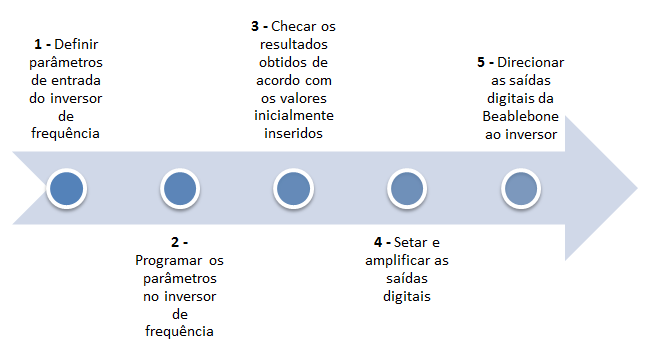
\includegraphics[width=1\textwidth]{inte02}
			\caption{Procedimento para realização do Teste de Integração Energia-Eletrônica}
			\label{inte02}
		\end{figure}

		Durante o teste, foram inicialmente utilizadas chaves seletoras que, a partir de uma lógica binária, selecionam as velocidades programadas pelos parâmetros do inversor de frequência. Em seguida substituiu-se as chaves seletoras pelas saídas digitais da Beaglebone. A Tabela \ref{inte03} apresenta as especificações do teste realizado.

		\begin{table}[!htpb]
		\centering
		\caption{Tabela de Teste - Valores de Entrada e Saída}
		\label{inte03}
		\begin{tabular}{|c|c|c|c|}
		\hline
		\rowcolor[HTML]{C0C0C0} 
		\multicolumn{3}{|c|}{\cellcolor[HTML]{C0C0C0}{\color[HTML]{000000} \textbf{\begin{tabular}[c]{@{}c@{}}Dados de entrada de acordo com a\\   lógica binária das caves seletoras\end{tabular}}}} & {\color[HTML]{000000} \textbf{Dados de saída}} \\ \hline
		\rowcolor[HTML]{C0C0C0} 
		{\color[HTML]{000000} \textbf{S1}} & {\color[HTML]{000000} \textbf{S2}} & {\color[HTML]{000000} \textbf{S3}} & {\color[HTML]{000000} \textbf{\begin{tabular}[c]{@{}c@{}}Velocidade do\\ inversor (rpm)\end{tabular}}} \\ \hline
		{\color[HTML]{000000} 1} & {\color[HTML]{000000} 1} & {\color[HTML]{000000} 0} & {\color[HTML]{000000} 300} \\ \hline
		{\color[HTML]{000000} 1} & {\color[HTML]{000000} 1} & {\color[HTML]{000000} 1} & {\color[HTML]{000000} 700} \\ \hline
		{\color[HTML]{000000} 1} & {\color[HTML]{000000} 0} & {\color[HTML]{000000} 0} & {\color[HTML]{000000} 800} \\ \hline
		{\color[HTML]{000000} 1} & {\color[HTML]{000000} 0} & {\color[HTML]{000000} 1} & {\color[HTML]{000000} 900} \\ \hline
		\end{tabular}
		\end{table}

	\section{Teste de Integração III - Equipes de Eletrônica e Software}
	\label{sec:inte33}

		Para a integração de todos os produtos, algumas áreas foram designadas para fazer sua integração de forma conjunta, é o caso da Equipe de Engenharia de Software e Equipe de Eletrônica.
		
		O objetivo deste teste de integração era estabelecer a comunicação da aplicação, a partir de um \textit{socket} e uma porta com endereços fixos, com o microcontrolador (\textit{beaglebone black}) e iniciar a execução do teste com base nos parâmetros inseridos pelo usuário na aplicação.
		
		Para realizar está integração, foram necessários os seguintes requisitos:

		\begin{itemize}
			\item as histórias de usuário US02, US03 e US07 completamente desenvolvidas e testadas;
			\item os módulos 2 (tratamento da comunicação) e 3 (controle da entrada e saída de dados), definidos com base na arquitetura proposta, completamente desenvolvidos e testados;
			\item o teste de integração entre acionamento do motor (Equipe de Energia) com o controle da entrada e saída de dados (Equipe de Eletrônica) completamente testado e aprovado.
		\end{itemize}

		O procedimento para realização do teste de integração e apresentado na Figura \ref{Imagem2}.
		\begin{figure}[htpb]
			\centering
			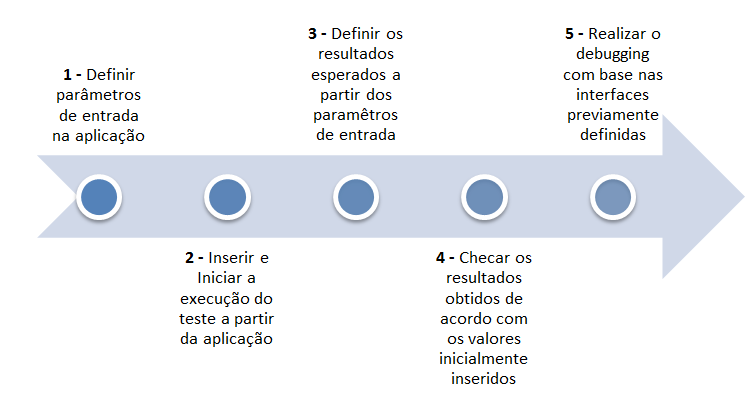
\includegraphics[width=1\textwidth]{Imagem2}
			\caption{Procedimento para realização do Teste de Integração Software-Eletrônica}
			\label{Imagem2}
		\end{figure}

		Por meio deste procedimento foi possível obter os resultados finais do teste de integração. O resultado seria dado como satisfatório quando todos os valores para o campo “resultados obtidos” estivessem de acordo com os valores de “resultados esperados”, os quais são definidos com base nos parâmetros de entrada. A Figura \ref{Imagem3} apresenta o plano de teste executado.
		\newpage
		\begin{figure}[htpb]
			\centering
			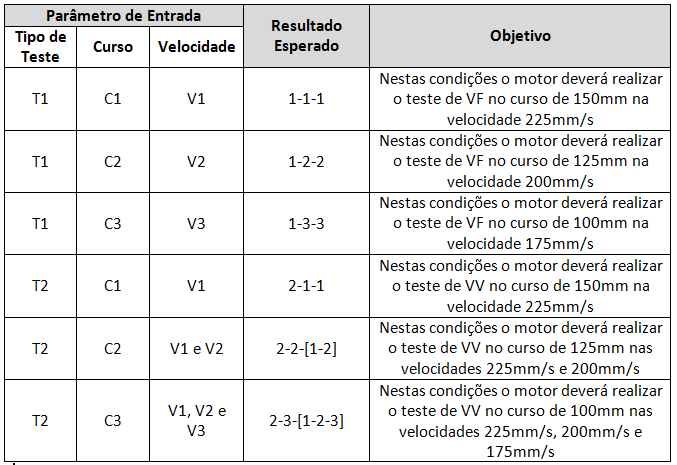
\includegraphics[width=1\textwidth]{Imagem3}
			\caption{Plano de Teste de Integração (Software-Eletrônica)}
			\label{Imagem3}
		\end{figure}

		Os valores T1 e T2 representam os tipos de testes de Velocidade Fixa (VF) e de Velocidade Variável (VV) respectivamente. Os valores C1, C2 e C3 representam Curso 1 (10cm), Curso 2 (12,5cm) e Curso 3 (15cm) respectivamente. Por fim, os valores V1, V2 e V3 representam Velocidade 1 (175mm/s), Velocidade 2 (200mm/s) e Velocidade 3 (225mm/s) respectivamente.

		Os resultados obtidos durante o experimento não serem inseridos neste relatório, pois não foram coletados de forma sistemática. Por fim, o resultado final do teste integração (software com eletrônica) foi dado com completo e satisfatório.

	\newpage
	\section{Custo Total do Projeto}
	\label{sec:inte44}

		Foram calculados os custos dos materiais utilizados para o desenvolvimento dos projetos de cada Engenharia. A Tabela \ref{custototal} apresenta o custo total de cada projeto.

		O cálculo dos custos não incluem o custo de desenvolvimento do software, tampouco das atividades de construção do produto, devido a não contabilização das horas empreendidas para tais atividades (essencial para cálculo da mão-de-obra empreendida) e nem os gastos com materiais não consumíveis como ferramentas, licenças, entre outros.
		
		\begin{table}[!htpb]
		\centering
		\caption{Custo Total do Projeto}
		\label{custototal}
		\begin{tabular}{|c|c|}
		\hline
		\rowcolor[HTML]{C0C0C0} 
		{\color[HTML]{000000} \textbf{Projeto}} & {\color[HTML]{000000} \textbf{Custo Total (R\$)}} \\ \hline
		{\color[HTML]{000000} Mecânico} & {\color[HTML]{000000} 1052,24} \\ \hline
		{\color[HTML]{000000} de Energia} & {\color[HTML]{000000} 119,00} \\ \hline
		{\color[HTML]{000000} Eletrônico} & {\color[HTML]{000000} 691,26} \\ \hline
		{\color[HTML]{000000} de Software} & {\color[HTML]{000000} 0,00} \\ \hline
		\rowcolor[HTML]{EFEFEF} 
		{\color[HTML]{000000} \textbf{Custo Total do Projeto (R\$)}} & {\color[HTML]{000000} \textbf{1862,50}} \\ \hline
		\end{tabular}
		\end{table}